\documentclass[]{article}
\usepackage[T1]{fontenc}
\usepackage[pdftex]{graphicx}
\graphicspath{ {./img/} }
\usepackage{graphicx}
%opening
\title{Book shop}
\renewcommand{\figurename}{Rys.}
\author{Kacper Wójcik, Marcin Stefaonwicz, Paweł Nowak}

\begin{document}

\maketitle

\begin{abstract}
	Book shop jest projektem sklepu internetowego z książkami. Głównym założeniem było stworzenie platformy przy użyciu Spring Boota z Mavenem, która pomoże użytkownikom w prowadzeniu sklepu internetowego. Aby wyizolować każdy element systemu, oraz aby u każdego programisty projekt działał tak samo został użyty Docker.

\end{abstract}
\newpage

\section{Projekt systemu}
\subsection{Kontenery}
System składa się z kilku dockerowych kontenerów stworzonych przy użyciu Docker Compose takich jak:
\begin{itemize}
	\item Spring App
	\item React
	\item PostgreSQL
\end{itemize}
\begin{figure}[h]
	\centering
	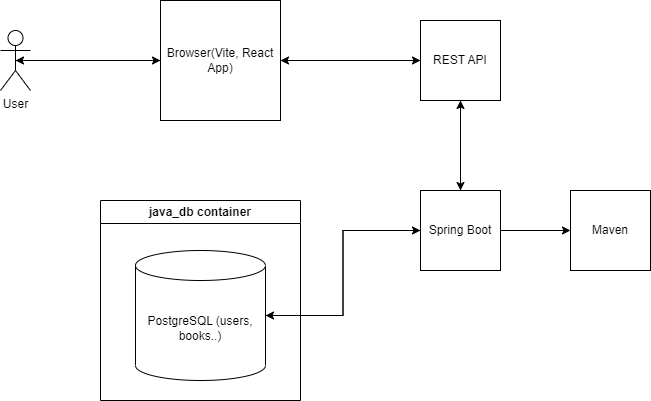
\includegraphics[scale=0.45]{ogolny_projekt.png}
	\caption{Ogólny projekt systemu}
\end{figure}
\subsubsection{Spring App}
Pierwszy kontener przechowuje główne elementy naszej aplikacji które łączą ze sobą kontenery np. REST API
\subsubsection{React}
\subsubsection{PostgreSQL}
Ostatni kontener przechowuje i pozwala zarządzać bazą danych PostgreSQL. Została wystawiona na port 5433, aby umożliwić wymianę danych między kontenerami, a jej zabezpieczenia np. możliwość stworzenia indywidualnych kont, oraz haseł pozwala zachować nam względne bezpieczeństwo. PostgreSQL został wybrany ze względu na jego popularność, szybkość działania, oraz to, że jest oparty na modelu relacyjnym.
Baza danych zawiera w aktualnej formie 6 tabel, którymi są:
\begin{itemize}
	\item Users
	\item Authors
	\item Orders
	\item OrderDetails
	\item Books
	\item BookCategories
\end{itemize}
\begin{figure}[h]
	\centering
	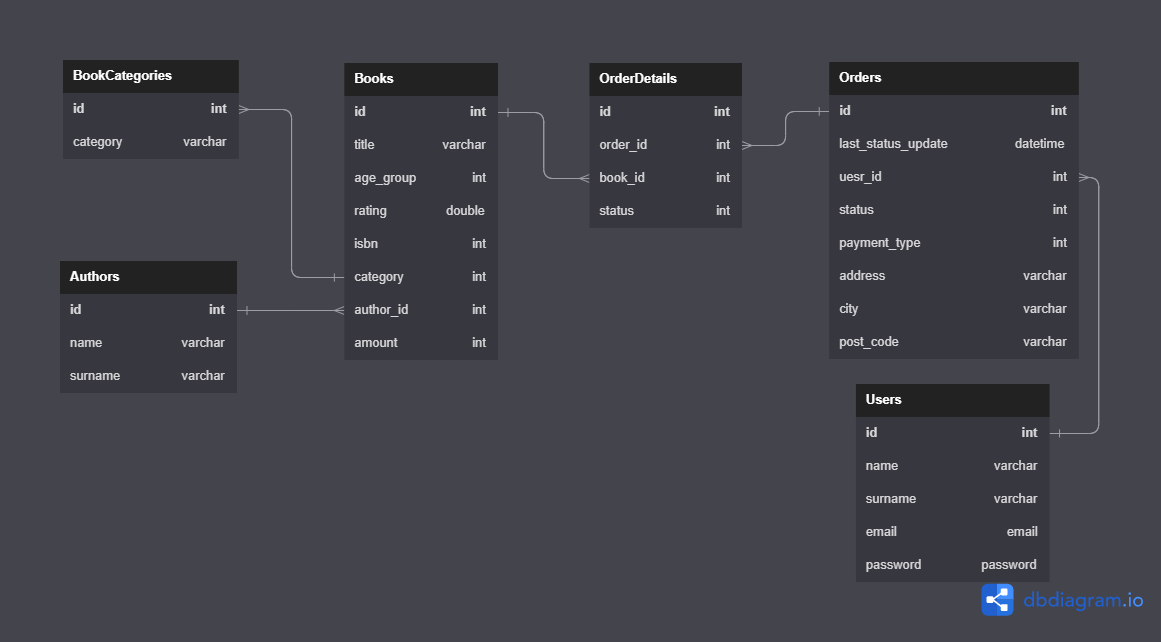
\includegraphics[scale=0.35]{../../DbDiagram.png}
	\caption{Projekt bazy danych}
\end{figure}

\subsection{Przypadki użycia}
Stworzony diagram przypadków użycia (Rys.3), przedstawia w sposób ogólny interakcje z aktorem(Userem), ramy systemu, oraz przypadki użycia. Użytkownik może stworzyć konto, zalogować się, przeglądać książki, a następnie po zalogowaniu zarządzać koszykiem tj. dodawać i usuwać książki z niego, lub przystąpić do zakupu.

\begin{figure}[h]
	\centering
	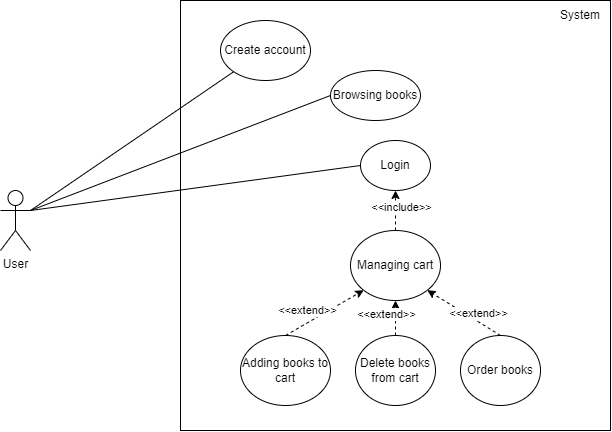
\includegraphics[scale=0.50]{przypadki_uzycia.png}
	\caption{Diagram przypadków użycia - User}
\end{figure}

Diagram przypadków użycia(Rys.4 Admin), przedstawia interakcje z aktorem(Adminem). Aktor może założyć konto, przeglądać książki. Po zalogowaniu dostaje możliwość zarządzania zamówieniami tj. zmiana statusu, realizacja itp., zarządzanie książkami, oraz nadawanie i odbieranie statusu admina innym użytkownikom.

\begin{figure}[ht]
	\centering
	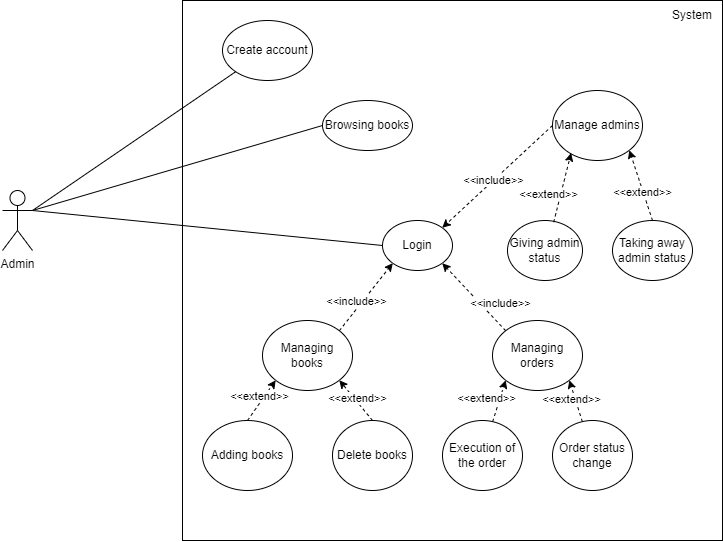
\includegraphics[scale=0.50]{przyp_uz_admin.png}
	\caption{Diagram przypadków użycia - Admin}
\end{figure}

Diagram aktywności logowanie/rejestracja(Rys.5) pokazuje proces rejestracji nowego użytkownika oraz proces logowania dla istniejących użytkowników. Zawierać weryfikację danych, oraz tworzenie konta użytkownika.
\begin{figure}[ht]
	\centering
	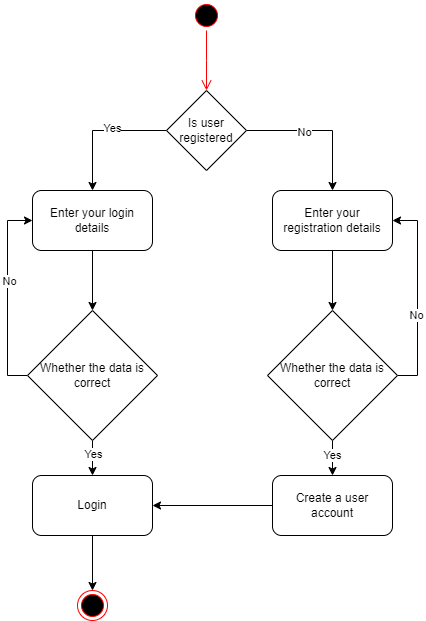
\includegraphics[scale=0.50]{log_rej.png}
	\caption{Diagram aktywności - logowanie/rejestracja}
\end{figure}

Diagram aktywności zakup książek(Rys.6) obejmuje kroki, które użytkownik podejmuje, aby dokonać zakupu książki. Obejmuje to wyszukiwanie książki, dodawanie jej do koszyka, przeglądanie koszyka, podawanie informacji o dostawie, wybór metody płatności, finalizację zamówienia itp.

\begin{figure}[ht]
	\centering
	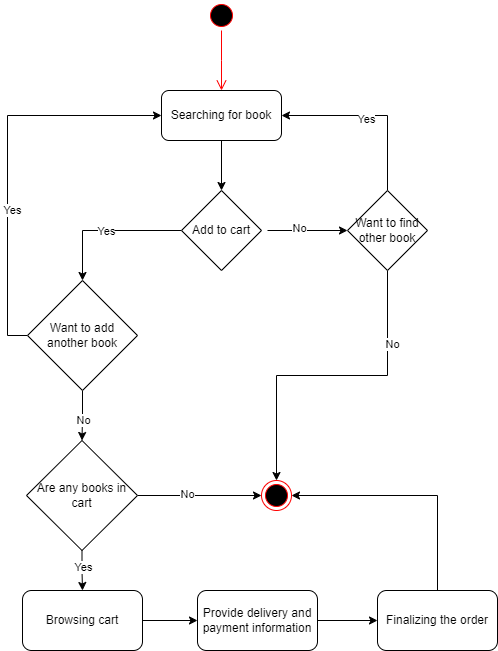
\includegraphics[scale=0.50]{zakup_ks.png}
	\caption{Diagram aktywności - zakup książek}
\end{figure}

Diagram aktywności obsługa zamówień(Rys.7), skupia się na obsłudze zamówień po ich złożeniu. Obejmuje akcje takie jak weryfikacja dostępności książki, przygotowanie książek, wysyłka i aktualizacja statusu zamówienia.

\begin{figure}[ht]
	\centering
	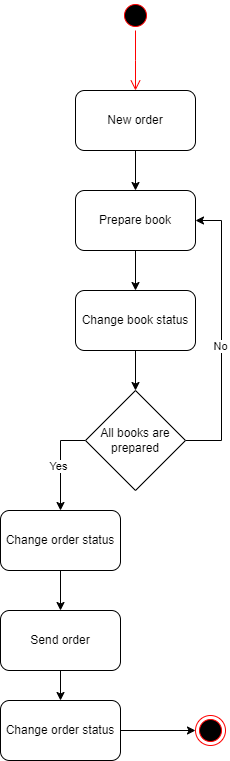
\includegraphics[scale=0.50]{obsl_zam.png}
	\caption{Diagram aktywności - obsługa zamówień}
\end{figure}



\end{document}
